\let\negmedspace\undefined
\let\negthickspace\undefined
\documentclass[journal]{IEEEtran}
\usepackage[a5paper, margin=10mm, onecolumn]{geometry}
%\usepackage{lmodern} % Ensure lmodern is loaded for pdflatex
\usepackage{tfrupee} % Include tfrupee package

\setlength{\headheight}{1cm} % Set the height of the header box
\setlength{\headsep}{0mm}     % Set the distance between the header box and the top of the text

\usepackage{gvv-book}
\usepackage{gvv}
\usepackage{cite}
\usepackage{amsmath,amssymb,amsfonts,amsthm}
\usepackage{algorithmic}
\usepackage{graphicx}
\usepackage{textcomp}
\usepackage{xcolor}
\usepackage{txfonts}
\usepackage{listings}
\usepackage{enumitem}
\usepackage{mathtools}
\usepackage{gensymb}
\usepackage{comment}
\usepackage[breaklinks=true]{hyperref}
\usepackage{tkz-euclide} 
\usepackage{listings}
% \usepackage{gvv}                                        
\def\inputGnumericTable{}                                 
\usepackage[latin1]{inputenc}                                
\usepackage{color}                                            
\usepackage{array}                                            
\usepackage{longtable}                                       
\usepackage{calc}                                             
\usepackage{multirow}                                         
\usepackage{hhline}                                           
\usepackage{ifthen}                                           
\usepackage{lscape}
\usepackage{tikz}
\usetikzlibrary{patterns}
\begin{document}


\bibliographystyle{IEEEtran}
\vspace{3cm}


\numberwithin{equation}{enumi}
\numberwithin{figure}{enumi}
\renewcommand{\thetable}{\theenumi}


% Marks the beginning of the document

\bibliographystyle{IEEEtran}
\vspace{3cm}


\title{2.6.10}
\author{AI25BTECH11004-B.JASWANTH}
% \maketitle
% \newpage
% \bigskip
{\let\newpage\relax\maketitle}


\renewcommand{\thefigure}{\theenumi}
\renewcommand{\thetable}{\theenumi}
\setlength{\intextsep}{10pt} % Space between text and floats

\textbf{Question}\\
Find the area of the triangle whose vertices are (-8,4),(-6,6) and (-3,9).\\
\textbf{Solution}:\\ 


\begin{table}[h!]
	\centering
	\begin{tabular}{|c|c|}
\hline
\textbf{Name} & \textbf{Value} \\ \hline
$\vec{A}$ & $\myvec{2 & 1 \\0 & 3}$ \\ \hline
\end{tabular}

	\caption{variables used}
	\label{}
\end{table}
\begin{align}
A-B = \myvec{-8 \\ 4} - \myvec{-6 \\ 6} 
= \myvec{-2 \\ -2},
\end{align}

\begin{align}
A-C = \myvec{-8 \\ 4} - \myvec{-3 \\ 9}
	= \myvec{-5 \\ -5}
 \end{align}




Now, the area of the triangle is
\begin{align}
 \text{ar}(\triangle ABC) 
= \frac{1}{2} \left| (A-B) \times (A-C) \right|   
\end{align}

\begin{align}
 \text{ar}(\triangle ABC)=  \frac{1}{2} \left| \myvec{-2 \\ -2} \times  \myvec{-5 \\ -5} \right |
\end{align}



\begin{align}
\therefore \quad \text{ar}(\triangle ABC) = \frac{1}{2}(0) = 0
\end{align}


\noindent
Thus, the three points are collinear, and the triangle has area=0.
\begin{figure}[h]
    \centering
    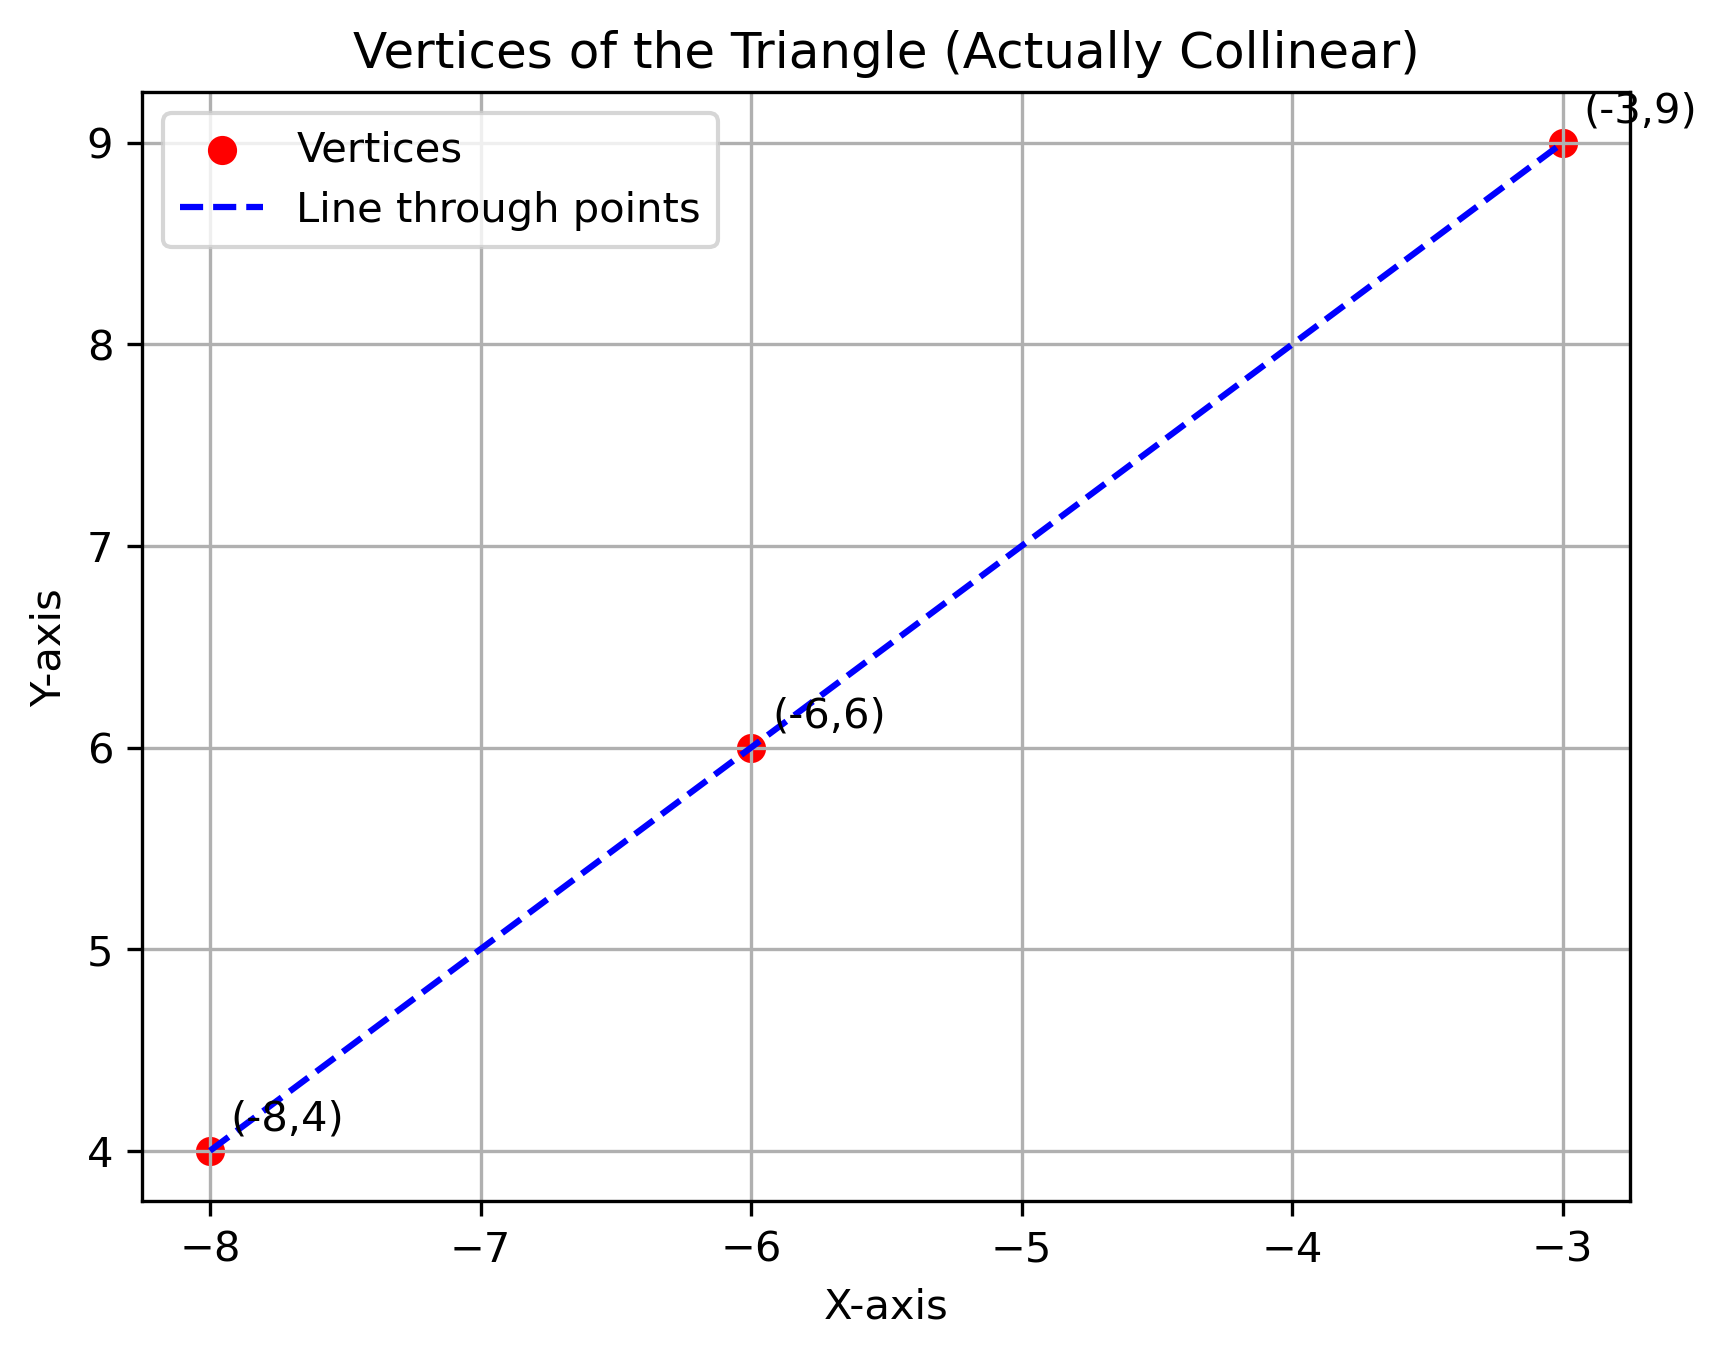
\includegraphics[width=0.9\linewidth]{figs/01.png}
    \caption{Caption}
    \label{fig:placeholder}
\end{figure}




\end{document}
